\chapter{Resumen Extendido}
%Debe incluir un resumen del trabajo de un máximo de 5 páginas. Resaltar aspectos fundamentales del desarrollo, los resultados más relevantes y las conclusiones.

El principal objetivo que persigue este trabajo fin de grado es mostrar y mejorar el sistema $ISA^{2}$ que presentaremos más adelante. Este sistema tiene como fin ser una alternativa para los ya existentes sistemas \ac{ISA}, puesto que éstos tienen una serie de fallos que solucionar y están enfocados de manera diferente.

La principal diferencia de $ISA^{2}$ con estos sistemas reside en cuál es la base de éste. Los sistemas \ac{ISA} están basados en tecnología \ac{GPS} y sensores de proximidad para con otros vehículos, mientras que la propuesta $ISA^{2}$ simplemente utiliza imágenes tomadas desde una cámara, y modelos de inteligencia artificial, para ser capaz de indicar al conductor la velocidad a la que debe circular.

En resumen, el sistema $ISA^{2}$ comienza capturando una imagen de la escena de tráfico que observa un vehículo. Sobre esta imagen se realiza un proceso de \ac{SS}. La \ac{SS} se puede explicar como el procedimiento de inteligencia artificial que es capaz de predecir qué clases (etiquetas) hay en una imagen, para cada uno de sus píxeles. Pero, ¿qué es una clase? O mejor dicho, ¿cómo definimos una clase en este contexto? Una clase (o etiqueta) es la forma de categorizar una parte de la imagen para diferenciarla de otras. Dicho de otra forma, sirve para que un programa sepa de qué partes se compone una imagen. Se hace dándole un mismo valor a un conjunto de píxeles en concreto, para distinguirlos de los demás \cite{deeplab}.

\begin{figure}[H]
  \centering
  \includegraphics[width=8cm]{Figuras/Ejemplo_Imagen_Segmentada.eps}
  \caption{Imagen Segmentada}
    \label{fig:ImgSegm}
\end{figure}

En la Figura \ref{ImgSegm} puede verse un ejemplo de segmentación semántica como la que utiliza nuestro modelo $ISA^{2}$. Una vez se ha completado la segmentación semántica, se utiliza esta información para entrenar un conjunto de regresores que son capaces de aprender a estimar la velocidad a la que debe ir el vehículo.

En este proyecto hacemos uso del modelo de deep learning \textbf{Swiftnet} \cite{swiftnet} para conseguir la segmentación semántica. \textbf{Swiftnet} es la base sobre la que desarrollamos este proyecto y donde más hemos trabajado para conseguir los resultados de las velocidades estimadas.

Swiftnet es un modelo de \textbf{tiempo real} que recibe imágenes de la vía cada cierto tiempo. Una vez las va recibiendo, va procesándolas una a una y predice una máscara de segmentación semántica en cada una de ellas, con una gran precisión.

Para trabajar con Swiftnet, previamente tenemos que construir el ``escenario'' sobre el que se va a ejecutar, y para ello nos servimos de un entorno \textbf{Conda} \cite{conda}. No entraremos, aún, en detalle sobre la explicación de Conda, pero sí diremos que nos sirve para crear un entorno virtual con todos los requerimientos necesarios para trabajar con Swiftnet.

Una vez lo creamos, siguiendo los pasos que más adelante explicaremos, conseguiremos replicar los resultado de Swiftnet tal y como se detallan en el artículo original \cite{swiftnet}, empleando el software que proporcionan los propios autores \cite{github_swiftnet}.

%Pero todavía no hemos terminado con Swiftnet, puesto que lo hemos ejecutado con una base de datos compuesta por imágenes que no se corresponde a la que se usó en la primera versión de $ISA^{2}$.

Una vez tenemos el modelo de segmentación semántica Swiftnet funcionando, pasamos a aplicarlo al problema propuesto. Por ello, debemos descargar la base de datos de $ISA^{2}$ y aplicar los cambios pertinentes en Swiftnet para que funcione en la misma, generando una máscara de segmentación semántica para cada imagen en $ISA^{2}$. Una vez lo conseguimos, debemos generar una serie de histogramas \cite{histograma} que recojan las clases de cada imagen procesada por Swiftnet, replicando el modelo propuesto en el artículo \cite{isa2}. Para generarlos nos serviremos de unos códigos en \textbf{MatLab} \cite{matlab}.

Con los histogramas creados, ya podemos ejecutar los sistemas de regresión para la parte final del proyecto: la estimación de la velocidad, y la comparación de la misma con la velocidad real de las imágenes (anotada en la base de datos $ISA^{2}$) . Todo esto lo hacemos replicando el modelo experimental descrito en \cite{isa2}, donde se proponen varias soluciones de inteligencia artificial para resolver el problema de la adaptación de la velocidad inteligente en base a imágenes.

\begin{figure}[H]
  \centering
  \includegraphics[width=8cm]{Figuras/Figura_Esquema_ISA2_Version_2.eps}
  \caption{Esquema $ISA^{2}$}
  \label{fig:isa2}
\end{figure}

En la figura \ref{isa2} puede verse la solución global propuesta, desde la segmentación semántica con Swiftnet hasta la aplicación del modelo de regresión para la estimación de la velocidad.

%TODO_DONE: Añade figura/diagrama explicativa de todo el sistema.

Según nuestros experimentos, los sistemas con mejores resultados, a pesar de que sean solo en entornos urbanos, son los que emplean \textit{Boosting Trees} \cite{boosting-trees} y \textit{\ac{SVR}} \cite{SVR}, como se puede ver en la tabla \ref{tab:Resul_Resumen}:

\begin{table}[H]
\centering
\resizebox{12cm}{!}{
\begin{tabular}{|l|l|l|l|l|}\cline{1-5}
& \multicolumn{2}{|l|}{\textbf{MAE Swiftnet}} & \multicolumn{2}{|l|}{\textbf{MAE DeepLab}} \\ \cline{1-5}
\textbf{Regresión} & \textbf{Highway (\%)} & \textbf{Urban (\%)} & \textbf{Highway (\%)} & \textbf{Urban (\%)}\\ \cline{1-5}
\textbf{\textit{Boosting Trees}} & 13.43 & \textbf{9.83} & 11.35 & \textbf{10.14} \\ \cline{1-5}
\textbf{\textit{SVR}} & 11.13 & \textbf{8.74} & 9.69 & \textbf{9.55} \\ \cline{1-5}
\end{tabular}
}
\caption{Resultados de Boosting Trees y \ac{SVR}}
\label{tab:Resul_Resumen}
\end{table}

En la tabla anterior hemos puesto los valores del \ac{MAE} más bajos, es decir, más precisos; calculados por dichos sistemas de regresión.

Nótese cómo particularmente en \textit{\ac{SVR}}, el margen de mejora con respecto a \textbf{DeepLab} (modelo usado en la primera versión) es de casi un 1\% (0.8\%). Por otro lado, \textit{Boosting Trees} es algo ``peor'' que \textit{\ac{SVR}} debido al poco margen de mejora que tiene (0.3\%).

Sin embargo, es importante destacarlo ya que el resto de sistemas son considerablemente menos precisos:

\begin{table}[H]
\centering
\resizebox{12cm}{!}{
\begin{tabular}{|l|l|l|l|l|}\cline{1-5}
& \multicolumn{2}{|l|}{\textbf{MAE Swiftnet}} & \multicolumn{2}{|l|}{\textbf{MAE DeepLab}} \\ \cline{1-5}
\textbf{Regresión} & \textbf{Highway (\%)} & \textbf{Urban (\%)} & \textbf{Highway (\%)} & \textbf{Urban (\%)}\\ \cline{1-5}
\textbf{\textit{Lasso}} & 12.90 & 9.23 & 11.29 & 8.43 \\ \cline{1-5}
\textbf{\textit{Linear}} & 12.22 & 8.95 & 10.32 & 8.38 \\ \cline{1-5}
\end{tabular}
}
\caption{Resultados de Lasso y Linear}
\label{tab:Resul_Resumen_LL}
\end{table}

Como se puede observar en la tabla \ref{tab:Resul_Resumen_LL}, tanto el sistema \textit{Lasso} como \textit{Linear} tienen buenos resultados en entornos urbanos, pero en comparación con DeepLab, no tienen un margen de mejora como tal. Dicho de otra forma, tienen un margen de mejora negativo.

A continuación podemos ver los resultados de las tablas gráficamente en las siguientes figuras:

\begin{figure}[H]
  \centering
  \begin{subfigure}[b]{0.45\linewidth}
    \includegraphics[width=\linewidth]{Figuras/Lineal_Highway(Nivel_1).eps}
    \caption{Highway con Linear}
  \end{subfigure}
    \begin{subfigure}[b]{0.425\linewidth}
    \includegraphics[width=\linewidth]{Figuras/Lasso_Highway(Nivel_1).eps}
    \caption{Highway con Lasso}
  \end{subfigure}
    \begin{subfigure}[b]{0.45\linewidth}
    \includegraphics[width=\linewidth]{Figuras/Boosting_Urban(Nivel_1).eps}
    \caption{Urban con Boosting Trees}
  \end{subfigure}
      \begin{subfigure}[b]{0.45\linewidth}
    \includegraphics[width=\linewidth]{Figuras/SVR_Urban(Nivel_1).eps}
    \caption{Urban con SVR}
  \end{subfigure}
  \caption{Resultados gráficos}
\end{figure}

Analizando estos resultados, vemos cómo los datos en los sistemas \textit{Lineal} y \textit{Lasso} son prácticamente idénticos. Esto es porque ambos están actuando en imágenes de autovías, donde Swiftnet no lo hace tan bien como DeepLab. En las tablas anteriores se puede ver cómo ésto no sólo es así usando estos dos sistemas, lo es para todos ellos, porque Swiftnet en ese tipo de entornos es peor que DeepLab.

No obstante, sí es mejor en un entorno en el que hay que tener una gran precisión para determinar qué elementos forman parte del mismo en cada momento: los núcleos urbanos.

Como se puede apreciar en las gráficas, la similitud entre la parte real (línea \textbf{azul}) y la estimada (línea \textbf{roja}) para los sistemas \textit{Boosting Trees} y \textit{\ac{SVR}} es más que evidente. Ambos sistemas son muy acertados para grandes urbes y cabría destacar más aún el propio \ac{SVR}, basándonos en los datos recogidos en la tabla \ref{tab:Resul_Resumen} y los mostrados en su gráfica. Que un sistema registre un \ac{MAE} tan bajo (8.74\%) para una zona urbana, denota que Swiftnet es el modelo adecuado para este proyecto.

%TODO_DONE: Añade más detalles sobre los números. Hay que resumir en un par de párrafos el capítulo de resultados.
%TODO_DONE: Añade resultados en gráficas.
%TODO_DONE: Añade resultados cualitativos.

De todos estos experimentos cabe destacar un hecho muy importante: Swiftnet, a diferencia de \textbf{DeepLab} (el modelo de \ac{SS} de la primera versión publicado en \cite{isa2}), es un modelo \textbf{Real-Time}, es decir, el coste de su implementación es mucho menor y, por si no fuera suficiente, trabaja mejor en entornos urbanos.

Por todo ello, y para concluir, podemos decir que: aunque DeepLab trabaje mejor en autovías y autopistas, Swiftnet lo compensa haciéndolo mejor en entornos urbanos, lo cual es más complejo por la dificultad que tiene el poder clasificar con gran precisión tan diferentes y variadas etiquetas en un mismo escenario. Además, cabe recordar que Swiftnet es un modelo Real-Time, de modo que la velocidad con la que procesa los datos es superior que la del modelo DeepLab (además del coste de implementación del propio modelo que ya hemos explicado con anterioridad). Finalmente, hemos visto la precisión en la estimación de la velocidad de Swiftnet observando las tablas y gráficas anteriores usando como métrica el \ac{MAE}, y se ha comprobado de forma cuantitativa cuánto mejor es éste con respecto a DeepLab para escenarios más complejos.
%TODO_DONE: Añade más conclusiones, sobre velocidad, precisión en la estimación, etc.
